\documentclass[lecture.tex]{subfiles}

\begin{document}

\exercice{Jessy Lefeuve}
%\video{https://youtu.be/blablabla}
\enonce{rdm-0017}{Etude en flexion}

Une poutre de longueur 3L et de section « en U inversé » est bi-appuyée en A et B (rotule ou pivot en A et appui ponctuel ou pivot glissant en B) et soumise à un effort F ponctuel au milieu du segment $A B$ et à un deuxième effort d'intensité $F$ en $C$ dans la direction $-\mathbf{y}$, tel que présenté sur le schéma ci-dessous.

\begin{center}
  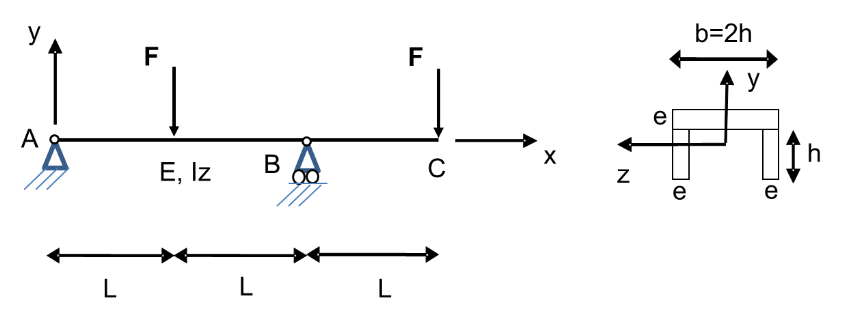
\includegraphics[scale=0.4]{figA0017.png}
\end{center}

\begin{enumerate}
  \item De quel type de flexion s’agit-il ?
  \item Trouver les efforts de liaison
  \item Trouver les efforts internes et tracer leurs évolutions en fonction de $x$
  \item Tracer l’évolution des contraintes $\sigma_{xx}$  en  fonction  de  $x$ pour  les  deux  surfaces hautes et basses de la poutre.
\end{enumerate}

\textbf{Données :}

\begin{itemize}
  \item[$\bullet$] Effort ponctuel : $F$
  \item[$\bullet$] Module d'Young : $E$
  \item[$\bullet$] Longueur : $L$
  \item[$\bullet$] Hauteur de la section : $h+e$
  \item[$\bullet$] Largeur de la section : $b=2h$
  \item[$\bullet$] Largeur des sous-sections rectangulaires : $e$
\end{itemize}

\medskip
\textbf{Nous allons éffectuer l'étude des contraintes.}

\medskip

\begin{enumerate}
  \item Déterminer le degré d’hyperstaticité du système.
  \item \'A l’aide d’une étude statique, déterminer les efforts de liaisons.
  \item Déterminer les efforts internes dans la poutre et tracer les diagrammes associés.
  \item Déterminer
  \begin{enumerate}
    \item la position du centre de géométrie
    \item le moment quadratique $I_z$ de la section de poutre.
    \item Sur un schéma d’une section à une abscisse quelconque de la poutre, localiser la contrainte normale maximale dans la poutre. Déterminer cette contrainte (en fonction de l'abscisse x).
    \item Pour les fibres supérieures et inférieures de la poutre (pour y maximal et y minimal), tracer l’évolution de la contrainte normale le long de la poutre en fonction de l’abscisse x.
    \item Donner la fonction d’évolution de la contrainte normale dans l’ensemble de la poutre en fonction des paramètres x et y.
    \item Déterminer et localiser la contrainte normale maximale de l’ensemble de la structure.
  \end{enumerate}

\end{enumerate}

\finenonce{rdm-0017}
\finexercice


\end{document}
